% !TEX encoding   = UTF8
% !TEX spellcheck = ru_RU
% !TEX root = ../seminars.tex

%%==================================================
\chapter{Представление программы на~машинном уровне}
%%==================================================

%%==========================
\section{Процесс компиляции}
%%==========================
\console/$ gcc -Og -o prog p1.c p2.c/%$

\noindent \GCC{} на~самом деле вызывает целый набор программ, чтобы перевести исходный код~\lang{С} в~исполняемый:

\medskip
\begin{itemfeature}
\item\emph{Препроцессор}. Расширяет исходный код, включая содержимое файлов, указанных посредством директивы \code{\#include}, и разворачивая макросы определяемые директивой \code{\#define}.

\item\emph{Компилятор}. Создаёт ассемблерные версии исходных файлов (\code{p1.s}, \code{p2.s}). Ключ (опция)~\hbox{\code{-Og}} предписывает компилятору использовать уровень оптимизации, при~котором получится машинный код, в~целом следующий общей структуре исходного кода на~\lang{C}. Использование более высоких уровней оптимизации (\code{-O1}, \code{-O2} и \code{-O3}) может привести к~генерации машинного кода, который настолько сильно изменён, что понять взаимосвязь с~исходным кодом затруднительно.

\item\emph{Ассемблер}. Переводит ассемблерный код в~объектный (\code{p1.o}, \code{p2.o}). Объектный код является одной из~форм машинного кода "--- он содержит двоичное представление всех команд, но адреса глобальных переменных ещё не определены.

\item\emph{Редактор связей}. Связывает объектные файлы между собой и с~библиотеками функций и создаёт файл \code{prog} (как предписывает ключ \code{-o}\,\code{prog}) с~исполняемым кодом. Исполняемые код "--- ещё одна форма машинного кода, которая может выполняться непосредственно процессором.
\end{itemfeature}



%%====================================
\section{Программа на~машинном уровне}
%%====================================
Компьютерные системы используют ряд абстракций, скрывая детали реализации и предоставляя более простую модель. Наиболее значимые абстракции:

\begin{itemfeature}
  \item \emph{Архитектура набора команд} (ISA "--- \textenglish{Instruction Set Architecture}). Определяет формат и представление программ на~машинном уровне.

  \item \emph{Виртуальные адреса памяти}. Позволяют представить память на~машинном уровне как очень большой массив байтов.
\end{itemfeature}

Ассемблерный код очень близок к~машинному. Основное отличие в~том, что язык ассемблера текстовый и более прост в~понимании для~человека.

Машинный код позволяет увидеть детали и части системы, которые скрыты от~программиста, пишущего на~языке~\lang{C}:

\begin{itemfeature}
  \item \emph{Счётчик команд}, обозначаемый \code{\%rip} в~\name{x86-64}. Определяет последовательность исполнения инструкций.

  \item Целочисленный \emph{файл регистров}. Содержит~16 именованных ячеек памяти для~хранения 64-битных значений. Эти регистры могут хранить адреса (соответствующие указателям в~\lang{C}) или целочисленные данные.

  \item Регистр флагов. Хранит информацию о~результатах последней выполненной арифметической или логической команды. Флаги используются для~реализации условных переходов (\code{if}, \code{while}, \ldots) и пересылки данных по~условию.

  \item Набор векторных регистров. Каждый может хранить одно или несколько целых чисел или чисел с~плавающей точкой.
\end{itemfeature}



\paragraph{Пример.} Рассмотрим следующий код, размещённый в~файле \code{mstore.c}:

\cfile{projects/sem05/mstore.c}

Ассемблерную версию этого кода можно получить, задав компилятору дополнительно ключик~\code{-S}:
\begin{consolecode}
$ gcc -Og -S mstore.c
$ vim mstore.s           # open file with the vim editor
\end{consolecode}

Команды листинга, начинающиеся с~точки, являются директивами ассемблера. Директивы вида \code{.cfi\_*} сохраняют дополнительную информацию, полезную при~отладке программ. Мы можем полностью их игнорировать. Для~отключения генерации этих директив, необходимо добавить ключик \code{-fno-asynchronous-unwind-tables}:

\console/$ gcc -Og -S -fno-asynchronous-unwind-tables mstore.c/%$

Набирать длинную команду каждый раз весьма утомительно. Для~неё можно объявить синоним (\textenglish{alias}):\label{alias:asmlst}

\console/$ alias asmlst="gcc -Og -S -fno-asynchronous-unwind-tables"/%$

\noindent и далее вызывать, используя новое имя:

\console/$ asmlst mstore.c/%$

\noindent В~результате получим ассемблерный листинг из~нашего кода на~\lang{C}:

\gasfile[firstline=5, lastline=11]{projects/sem05/mstore.s}

Ключ~\code{-c} предписывает \GCC{} выполнить и компиляцию, и ассемблирование:

\console/$ gcc -Og -c mstore.c/%$

\noindent Таким образом получается объектный файл (\code{mstore.o}). С помощью отладчика:

\console/$ gdb mstore.o/%$

\noindent можно увидеть машинный код инструкций функции:

\textfile[firstline=16]{projects/sem05/gdb.sh-session}

\noindent Отсюда понятно, что программа, выполняемая машиной,~--- это всего лишь последовательность байтов, кодирующих серию машинных инструкций.

Исследовать содержимое файлов с машинным кодом можно при помощи программ называемых \emph{дизассемблерами}:

\console/$ objdump -d mstore.o/%$

\noindent Из~машинного кода они создают код в~формате похожем на~ассемблерный листинг:

\objdumpfile[firstline=6, lastline=13]{projects/sem05/mstore.c-objdump}

Следует отметить, что:
\begin{itemfeature}
  \item Инструкции \name{x86-64} имеют переменную длину от~1 до~15 байт. Код устроен так, что часто используемые инструкции, а также те, что имеют меньшее количество операндов, занимают меньше байтов.

  \item Формат спроектирован так, что инструкцию можно однозначно декодировать, начиная с~некоторой фиксированной позиции.

  \begin{figure}[h]
    {\centering
      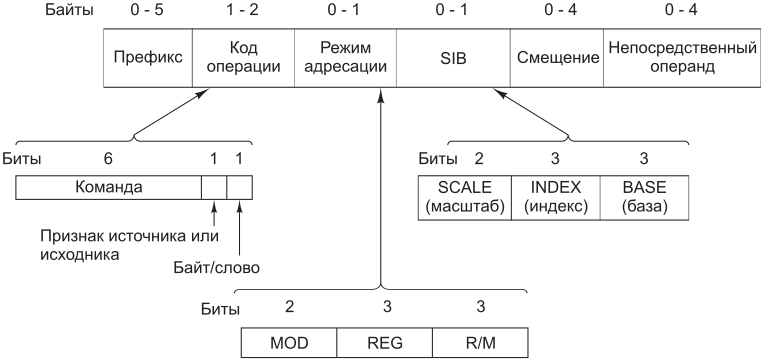
\includegraphics[width=0.8\textwidth]{images/command_format_corei7.png}

    }
    \caption{Формат команд процессора \name{Core}\,\name{i7}}
    \label{fig:cmd:corei7}
  \end{figure}

  \item Дизассемблер выводит ассемблерный код, исходя только из~последовательности байтов в~файле с~машинным кодом.

  \item Дизассемблер использует немного иные соглашения об~именовании, чем \GCC. В~частности, он опускает суффукс~\code{q} у~многих инструкций.
\end{itemfeature}

Чтобы создать код, который будет выполняться системой, необходимо запустить \emph{компоновщик} для~набора объектных файлов, в~одном из~которых определена функция \code{main} (\code{main.cpp}):

\cfile{projects/sem05/main.cpp}

Директива \code{extern "C"} предписывает компилятору использовать соглашения языка~\lang{C} для~именования функций. Язык~\lang{C++} поддерживает <<перегрузку>> имени функции и, вследствие этого, придерживается иных правил об~именовании: он выполняет декорацию (\textenglish{mangling}) исходного имени при~помощи имён типов аргументов.

Собрать исполняемый код можно командой:

\console/$ g++ -Og -o prog main.cpp mstore.o/%$

Объём исполняемого файла значительно больше объёма составляющих его объектных файлов, поскольку он содержит не только код наших процедур, но также информацию, необходимую для~запуска и завершения программы и для~взаимодействия с~операционной системой. Выполнив команду:

\console/$ objdump -d prog/%$

\noindent получим дизассемблерный листинг исполняемого кода:

\objdumpfile[firstline=143, lastline=149]{projects/sem05/prog.c-objdump}

\noindent Какие изменения произошли в~коде функции \code{multstore} при~компоновке?



%%================
\WhatToReadSection
%%================
\citeauthor[глава~3, стр.~190--197]{Bryant:2022:ru}



%%===============
\ExercisesSection
%%===============
\begin{exercise}
\item Настройте рабочую среду, следуя инструкциям из~соответствующего подраздела на~странице~\pageref{sect:workEnv}, если Вы не сделали этого ранее.


\item Рассмотрим следующий код, который пытается просуммировать элементы массива \code{arr}, количество элементов задаётся параметром \code{length}:
\begin{ccode}
/* WARNING: This is buggy code */
float sum_elements (float arr[], unsigned length)
{
  float result = 0.;
  for (int i = 0; i <= length - 1; ++i)
    result += arr[i];

  return result;
}
\end{ccode}

Если вызвать функцию с~аргументом \code{length}, равным \code{0}, то она должна вернуть нуль. Однако вместо этого происходит ошибка при~работе с~памятью. Объясните, почему. Покажите, как исправить код.


\item Рассмотрим следующие \lang{C}-функции:
\begin{ccode}
int fun1 (unsigned word)
{
  return (int) ((word << 24) >> 24);
}

int fun2 (unsigned word)
{
  return ((int) word << 24) >> 24;
}
\end{ccode}

Положим, что они выполняются под~управлением 32-разрядной машины, которая использует арифметику на~основе дополнения до~двух. Также положим, что сдвиг вправо для~чисел со~знаком выполняется арифметически, а для~чисел без~знака "--- логически.
\begin{enumIssue}
  \item Заполните таблицу ниже, которая показывает действие функций на~примере нескольких аргументов. Будет удобнее работать с~числами в~шестнадцатеричной записи. Помните, что цифры от~\code{8} до~\code{F} имеют старший бит равный~\code{1}.

  \begin{flushleft}\ttfamily\small\newcommand*{\ans}{\ansvw}\begin{tabular}{@{}ccc@{}}
    w          & fun1(w)          & fun2(w) \\
    \midrule
    0x00000076 & \ans{0x00000076} & \ans{0x00000076} \\
    0x87654321 & \ans{0x00000021} & \ans{0x00000021} \\
    0x000000C9 & \ans{0x000000C9} & \ans{0xFFFFFFC9} \\
    0xEDCBA987 & \ans{0x00000087} & \ans{0xFFFFFF87} \\
  \end{tabular}\end{flushleft}

  \item Опишите словами, какое полезное вычисление выполняет каждая из~функций.
\end{enumIssue}


\item Вам дали задание написать функцию, которая определяет длиннее ли одна строка, чем другая. Вы решили использовать стандартную функцию \code{strlen}, которая объявляется следующим образом:
\begin{ccode}
/* Prototype for library function strlen */
size_t strlen (const char *s);
\end{ccode}

Вот первая попытка:
\begin{ccode}
/* Determine whether string s is longer than string t */
/* WARNING: This function is buggy */
int strlonger (char *s, char *t)
{
  return strlen(s) - strlen(t) > 0;
}
\end{ccode}

Во время тестирования на~некоторых данных результаты получились неправильные. Вы занялись отладкой и выяснили, что при~компиляции для~32-разрядной архитектуры тип данных \code{size\_t} определён (через \code{typedef}) в~заголовочном файле \code{stdio.h} как \code{unsigned}.
\begin{enumIssue}
  \item В~каких случаях функция выдаёт неверный результат?
  \item Объясните, каким образом этот неверный результат получается.
  \item Покажите, как исправить код, чтобы он работал надёжно.
\end{enumIssue}


\newcommand*{\lstitem}[1]{%
  \makebox[1.5em][r]{\textrm{#1.}}%
}
% O'Hallaron, 3rd ed., problem 2.18
\item Нам будут встречаться листинги, генерируемые дизассемблером "--- программой, которая преобразует исполняемый файл обратно в~более читабельную ASCII форму. Эти файлы содержат много шестнадцатеричных чисел, обычно представленных в~виде дополнения до~двух. Способность распознавать эти числа и понимать их смысл (например, положительные они или отрицательные) представляет собой важный навык.

Преобразуйте шестнадцатеричные значения (в~32-битном дополнении до~двух), представленные в~листинге справа от~мнемоник команд (\code{sub}, \code{mov} и \code{add}) в~десятичные эквиваленты:

{\newcommand*{\ans}{\hfill\ansvw}%
  \objdumpfile[linenos=false, escapeinside=||]{projects/sem05/some_code.c-objdump}
}


% O'Hallaron, 3rd ed., problem 2.44
\item Положим, что \code{int} занимает 32 бита и использует дополнение до~двух для~представления чисел со~знаком. Сдвиги вправо выполняются арифметически для~значений со~знаком и логически для~значений без~знака. Переменные объявлены и инициализированы следующим образом:
\begin{ccode}
int x = foo();  /* Arbitrary value */
int y = bar();  /* Arbitrary value */

unsigned ux = x;
unsigned uy = y;
\end{ccode}

Для~каждого из~следующих~\lang{C} выражений докажите, что оно истинно для~всех значений~\code{x} и~\code{y}, или приведите значения~\code{x} и~\code{y}, для~которых оно ложно:
{\newcommand*{\ans}{\hfill\ansfw{7em}}%
\begin{ccode*}{linenos=false, escapeinside=zz}
  z\lstitem{А}z (x > 0) || (x - 1 < 0) z\ans{min int32\_t}z
  z\lstitem{Б}z (x & 7) != 7 || (x << 29 < 0) z\ans{true}z
  z\lstitem{В}z x * x >= 0 z\ans{0xFFFF}z
  z\lstitem{Г}z x < 0 || -x <= 0 z\ans{true}z
  z\lstitem{Д}z x > 0 || -x >= 0 z\ans{min int32\_t}z
  z\lstitem{Е}z x + y == uy + ux z\ans{true}z
  z\lstitem{Ж}z x * ~y + uy * ux == -x z\ans{true}z
\end{ccode*}
}

\end{exercise}
